\documentclass[11pt]{article}
\usepackage[utf8]{inputenc} 
\usepackage[T1]{fontenc}
\usepackage{sectsty}
\usepackage{graphicx}
\usepackage{amsmath}
\usepackage{booktabs}
\usepackage{placeins}

% Margins
\topmargin=-0.45in
\evensidemargin=0in
\oddsidemargin=0in
\textwidth=6.5in
\textheight=9.0in
\headsep=0.25in

\title{ HAFiscal project paper outline}
\author{Christopher Carroll, Edmund Crawley, Ivan Frankovic, Håkon Tretvoll}
\date{\today}

\begin{document}
	\maketitle
	
	
	\section{Introduction}
	
	\section{Model}
	
	\section{Estimation and calibration}
	
	\subsection{Estimation of the "splurge" factor}
	
	There is much evidence from analysis of micro data, that people tend to "splurge" on changes to their income. We defining splurging as the free spending of available income without concern for intertemporal maximization of utility. As we will show, a model allowing for splurging performs well at capturing the shorter and longer term response of consumption to income shocks.
	
	\paragraph{Lottery experiment Fagereng et al.}
	
	TO DO: Cite paper correctly, look up how results are presented in other papers by Chris.
	

	\paragraph{Targets} In this section we estimate the splurge factor, the mean discount rate across the population as well as its spread to match two empirical moments. 
	
	First, we match the steady-state distribution of liquid wealth in the model to its empirical counterpart. Due to the lack of data on the liquid wealth distribution in Norway, we resort to the corresponding data from the US - assuming that liquid wealth inequality is comparable across these countries. Specifically, we impose as targets the cummulative liquid wealth share at the 20th, 40th, 60th and 80th income percentile, which equal 0\%, 0.4\%, 2.5\% and 11.7\%. Hence, 87.3\% of the total liquid wealth is  held by the top income quintile. The data is plotted in figure \ref{fig:liquwealthdistribution}.
	\begin{figure}
		\centering
		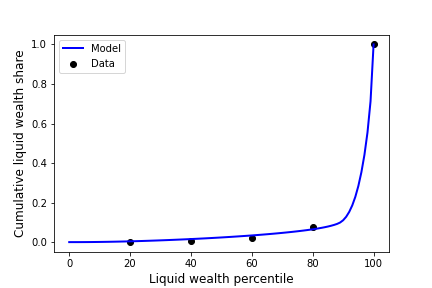
\includegraphics[width=0.8\linewidth]{../Code/HA-Models/Target_AggMPCX_LiquWealth/Figures/LiquWealth_Distribution}
		\caption{Distribution of liquid wealth across income groups}
		\label{fig:liquwealthdistribution}
	\end{figure}
	Second, we take from Fagereng et al. the marginal propensity to consume out of a one-period income shock. We not only target the contemporaneous respone of consumption to the income shock, but also the subsequent impact on consumption in years one to four after the income shock. The MPCs from Fagereng et al. are plotted in figure \ref{fig:aggmpclotterywin}.
	\begin{figure}
		\centering
		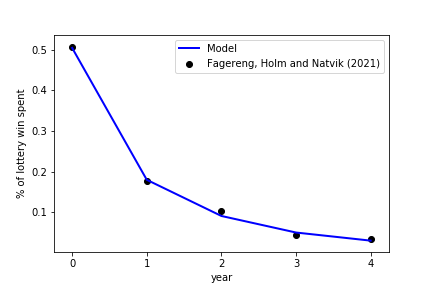
\includegraphics[width=0.8\linewidth]{../Code/HA-Models/Target_AggMPCX_LiquWealth/Figures/AggMPC_LotteryWin}
		\caption{Aggregate marginal propensity to consume in response to a lottery in year zero}
		\label{fig:aggmpclotterywin}
	\end{figure}
	
	\paragraph{Parameterization}
	
	To do: Look up the calibration source for each of these moments, possibly email Chris and Edmund about it
	
	\begin{itemize}
		\item LivPrb, Source?
		\item Rfree, UnemPrb from NORA
		\item IncUnemp, Source?
		\item PermShkStd, TransShkStd, Source?
		\item BoroCnstArt is set to -0.8. This means the borrowing constraing amounts to 80\% of quartarly permanent income, hence 20\% of year permanent income.  Source ?		
		\item PermGroFacAgg is set to 1.5\%, Source?
		\item Tage, Tsim 
	\end{itemize}

	
	\section{Fiscal policy simulations}
	
	We consider the following fiscal policy experiments
	
	\begin{itemize}
		\item Payroll tax cut: Employed individuals benefit from a 2 percentage points lower payroll tax cut. The tax cut is unanticipated and usually lasts for 8 quarters. However, there is a 50\% chance, that the policy is extended by another 8 quarters if the recession is still ongoing in the 8th quarter of the payroll tax cut. 
		\item Unemployment insurance extension: The duration of the unemployment insurance is doubled from 2 to 4 quarters. Agents, that are unemployed when the policy is implemented thus receive up to 4 quarters of unemployment insurance. The policy is unanticipated and active only for one quarter.
		\item Stimulus check: Each individual, independent of employment status, receives an unanticipated payment of \$1200 in one quarter. However, the check is only paid out fully to individuals with a permanent yearly income smaller than 100,000 and not at all to those with a income greater than 150,000. Those within the two thressholds receive a share of the full stimulus check amount proportionate to their position within threshholds.\footnote{For this income group, the check amount is given by $\$1200 (1-\frac{Income-100,000}{50,000})$. For example, an individual with a permanent yearly income of 110,000 receives 80\% of the stimulus, i.e. \$960.}
	\end{itemize}
	
	\subsection{Impulse responses}
	
	
	\begin{figure}
		\centering
		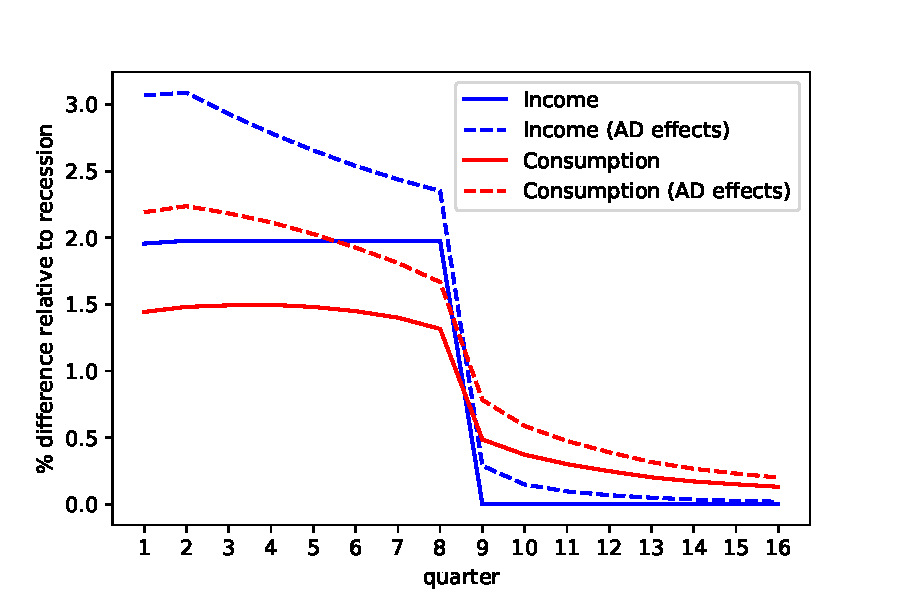
\includegraphics[width=0.8\linewidth]{../Code/HA-Models/FromPandemicCode/Figures/recession_taxcut_relrecession}
		\caption{Impulse responses of aggregate income and consumption to a pay roll tax cut during a recesssion lasting eight quarters with and without aggregate demand effects}
		\label{fig:recessiontaxcutrelrecession}
	\end{figure}
	
	\begin{figure}
		\centering
		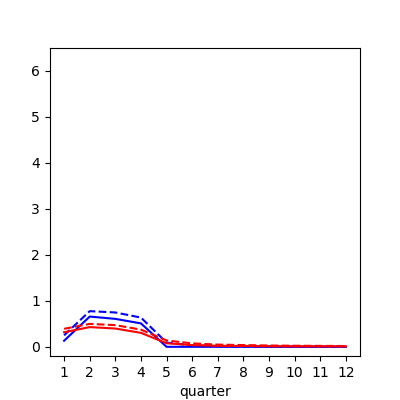
\includegraphics[width=0.8\linewidth]{../Code/HA-Models/FromPandemicCode/Figures/recession_UI_relrecession}
		\caption{Impulse responses of aggregate income and consumption to a UI extension during a recesssion with and without aggregate demand effects}
		\label{fig:recessionuirelrecession}
	\end{figure}
	
	\begin{figure}
		\centering
		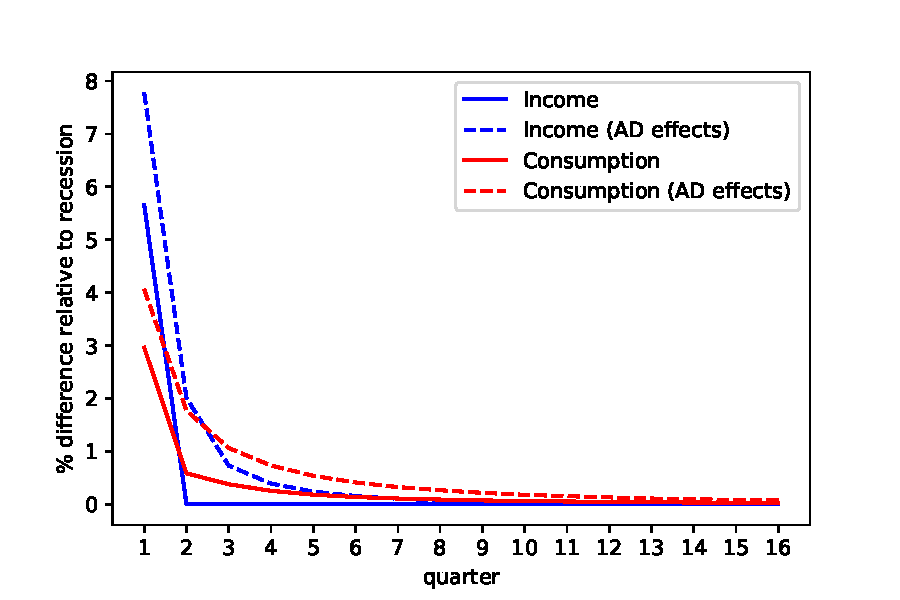
\includegraphics[width=0.8\linewidth]{../Code/HA-Models/FromPandemicCode/Figures/recession_Check_relrecession}
		\caption{Impulse responses of aggregate income and consumption to a stimulus check during a recesssion with and without aggregate demand effects}
		\label{fig:recessioncheckrelrecession}
	\end{figure}

	\FloatBarrier
	\subsection{Multipliers}
	
	Definitions:
	\begin{itemize}
		\item The \textit{net present value (NPV)} of a variable X at horizon t is given by
		\begin{equation}
			NPV(t,X) = \sum_{s=0}^{t} \left( \prod_{i=1}^{s} \frac{1}{R_i} \right) X_s
		\end{equation}
		\item The \textit{cummulative multiplier (CM)} of a policy is given by
		\begin{equation}
			CM(t) = \frac{NPV(t,\Delta C)}{NPV (T_{max},\Delta G)}
		\end{equation}
		where $\Delta C$ is the additional aggregate consumption spending in the policy scenario relative to the baseline and $\Delta G$ is the government expenditures caused by the policy.
	\end{itemize}
	
	\begin{table} 
		\center
		\input ../Code/HA-Models/FromPandemicCode/Tables/Multiplier.tex
		\caption{Multipliers as well as the share of the policy ocurring during the recession for the three policies considered}
		\label{tab:Multiplier}
	\end{table}

	\begin{table} 
		\center
		\input ../Code/HA-Models/FromPandemicCode/Tables/Multiplier_RecLengths.tex
		\caption{Multipliers (with AD effects) for different recesssion lengths for the three policies considered}
		\label{tab:Multiplier_RecLengths}
	\end{table}
	
	\begin{figure}
		\centering
		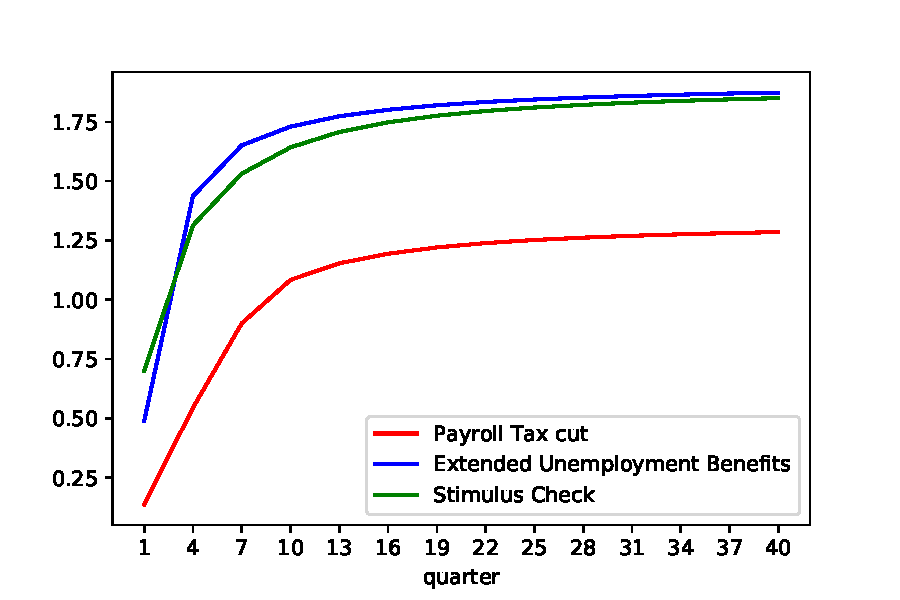
\includegraphics[width=0.8\linewidth]{../Code/HA-Models/FromPandemicCode/Figures/Cummulative_multipliers}
		\caption{Cummulative Multiplier as a function of the horizon in quarters for the three policies considered. Policies are implemented during a recession with AD effects active}
		\label{fig:cummulativemultipliers}
	\end{figure}
	
	\FloatBarrier
	\section{Welfare analysis}
	
	We want to convert welfare units to consumption units. A proportional increase in every agents' consumption in the baseline by fraction $x$, in welfare, is equal to:
	\begin{align}
	x\frac{1}{N}\sum_{i=1}^{N} \sum_{t=0}^{\infty} D^t c_{it,\text{base}} u'(c_{it,\text{base}})
	\end{align}
	where $c_{it}$ is consumption (including the splurge) of agent $i$ at time $t$ and $D$ is the social planner's discount rate. $N$ is the number of agents.
	
	
	The cost of such an increase is
	\begin{align}
	x\frac{1}{N}\sum_{i=1}^{N} \sum_{t=0}^{\infty} R^{-t} c_{it,\text{base}}
	\end{align}
	Define
	\begin{align}
	\mathcal{W}^c =\frac{1}{N}\sum_{i=1}^{N} \sum_{t=0}^{\infty} D^t c_{it,\text{base}} u'(c_{it,\text{base}}) \\
	\mathcal{P}^c = \frac{1}{N}\sum_{i=1}^{N} \sum_{t=0}^{\infty} R^{-t} c_{it,\text{base}}
	\end{align}
	Aside - with log utility, $\mathcal{W}^c =\frac{1}{N}\sum_{i=1}^{N} \sum_{t=0}^{\infty} D^t = \frac{1}{1-D}$
	
	We will assume that a government expenditure of size $F$ with welfare benefit $\mathcal{W}$ will be funded by a proportional consumption tax of size $\frac{F}{\mathcal{P}^c}$ resulting in a welfare loss of $\frac{F}{\mathcal{P}^c}\mathcal{W}^c$. The overall welfare benefit will be equivalent to consumption units:
	\begin{align}
	\mathcal{C} = \frac{\mathcal{W}}{\mathcal{W}^c} - \frac{F}{\mathcal{P}^c}
	\end{align}
	There is also an `unseen' cost to the government policy exactly equal to implementing the policy in normal times.
	
	Define welfare of a policy as:
	\begin{align}
	\mathcal{W}(\text{policy},AD,Rec) = \frac{1}{N}\sum_{i=1}^{N} \sum_{t=0}^{\infty} D^t u(c_{it,\text{policy},AD,Rec})
	\end{align}
	
	So the consumption equivalent of a policy implemented in recession is:
	\begin{align}
	\mathcal{C}(\text{policy},AD,Rec) &= \bigg(\frac{\mathcal{W}(\text{policy},AD,Rec)-\mathcal{W}(AD,Rec)}{\mathcal{W}^c} - \frac{PV(\text{policy},Rec)}{\mathcal{P}^c} \bigg)\\ \nonumber
	& \qquad -
	\bigg(\frac{\mathcal{W}(\text{policy}) - \mathcal{W}(\text{base})}{\mathcal{W}^c} - \frac{PV(\text{policy})}{\mathcal{P}^c} \bigg)
	\end{align}
	
	\begin{table} 
		\center
		\input ../Code/HA-Models/FromPandemicCode/Tables/welfare4.tex
		\caption{Consumption Equivalent Welfare Gains in Basis Points }
		\label{welfare}
	\end{table}
	
	Table \ref{welfare} shows results for this method. Note that the policy expenditures of each policy have been equalized.
	
	\section{Conclusion}
	
	\appendix
	\section{Appendix section example}
	
	
	
\end{document}